\section{Auswertung}
\label{sec:Auswertung}

Die Messung wird nach \autoref{sec:Durchführung} durchgeführt. Die Messwerte werden in \autoref{tab:Messung1} dargestellt.

%\begin{table}[H]
 %   \centering
  %  \caption{Messwerte des Millikan-Versuchs.}
   % \label{tab:Messung1}
   % \sisetup{table-format=2.2}
    \begin{longtable}{ S[table-format=3.1]S[table-format=1.3]SS  S S S }
    \caption{Messwerte des Millikan-Versuchs.}\label{tab:Messung1}\\
    \toprule
    {$U / \si{\volt}$} & {$R / \si{\mega\ohm}$}&  {$t_0 / \si{\second}$} & \multicolumn{2}{c}{$t_{auf} / \si{\second}$} &\multicolumn{2}{c} {$t_{ab} / \si{\second}$} \\
    \midrule
    \endfirsthead
    \caption{(fortgesetzt)}\\
    {$U / \si{\volt}$} & {$R / \si{\mega\ohm}$}&  {$t_0 / \si{\second}$} & \multicolumn{2}{c}{$t_{auf} / \si{\second}$} &\multicolumn{2}{c} {$t_{ab} / \si{\second}$} \\
    \midrule
    \endhead    
    243.4   &   2.023 &  11.12  &  \multicolumn{2}{c} {$2.75$}    &  \multicolumn{2}{c} {$4.78$}    \\
            &         &         &   \multicolumn{2}{c} {$3.43$}   &                                  \\
    \midrule
      {Mittelwert}& &  & \multicolumn{2}{c}{$3.09 \pm 0.34$}& \multicolumn{2}{c} {$4.78$}\\
    \midrule
    \pagebreak[1]
    243.4   &   2.023  &   27.76   &  \multicolumn{2}{c} {$13.22$}   &  \multicolumn{2}{c} {$5.43$}    \\
            &          &           &  \multicolumn{2}{c} {$12.36$}   &  \multicolumn{2}{c} {$5.44$}    \\
            &          &           &  \multicolumn{2}{c} {$13.62$}   &  \multicolumn{2}{c} {$5.14$}    \\
            &          &           &  \multicolumn{2}{c} {$12.24$}   &  \multicolumn{2}{c} {$5.92$}    \\
    \midrule
      {Mittelwert}& &  & \multicolumn{2}{c}{$12.86 \pm 0.33$}& \multicolumn{2}{c} {$5.48 \pm 0.16$}\\
    \midrule
    \pagebreak[1]
    242.4   &   1.992  &   16.60   &  \multicolumn{2}{c} {$5.45 $}   &  \multicolumn{2}{c} {$3.76$}    \\
            &          &           &  \multicolumn{2}{c} {$5.67 $}   &  \multicolumn{2}{c} {$3.58$}    \\
            &          &           &  \multicolumn{2}{c} {$5.71 $}   &  \multicolumn{2}{c} {$3.41$}    \\
    \midrule
    {Mittelwert}& &  & \multicolumn{2}{c}{$5.61 \pm 0.08$}& \multicolumn{2}{c} {$3.58 \pm 0.10$}\\
    \midrule
    \pagebreak[1]
    242.3   &   1.990  &   22.24   &  \multicolumn{2}{c} {$4.65 $}   &  \multicolumn{2}{c} {$4.43$}    \\
            &          &           &  \multicolumn{2}{c} {$5.49 $}   &  \multicolumn{2}{c} {$4.17$}    \\
            &          &           &  \multicolumn{2}{c} {$3.69 $}   &  \multicolumn{2}{c} {$3.90$}    \\
    \midrule
    {Mittelwert}& &  & \multicolumn{2}{c}{$4.61 \pm 0.52$}& \multicolumn{2}{c} {$ 4.17 \pm 0.15$}\\
    \midrule
    \pagebreak[1]
    242.2   &   1.986  &   23.82   &  \multicolumn{2}{c} {$5.32 $}   &  \multicolumn{2}{c} {$4.23$}    \\
            &          &           &  \multicolumn{2}{c} {$5.85 $}   &  \multicolumn{2}{c} {$4.24$}    \\
            &          &           &  \multicolumn{2}{c} {$6.37 $}   &  \multicolumn{2}{c} {$4.13$}    \\
    \midrule
    {Mittelwert}& &  & \multicolumn{2}{c}{$5.85 \pm 0.30$}& \multicolumn{2}{c} {$4.13\pm 0.06$}\\
    \midrule
    \pagebreak[1]
    199.3   &   1.980  &   21.82   &  \multicolumn{2}{c} {$5.20 $}   &  \multicolumn{2}{c} {$3.47$}    \\
            &          &           &  \multicolumn{2}{c} {$5.89 $}   &  \multicolumn{2}{c} {$3.53$}    \\
            &          &           &  \multicolumn{2}{c} {$5.86 $}   &  \multicolumn{2}{c} {$3.94$}    \\
    \midrule
    {Mittelwert}& &  & \multicolumn{2}{c}{$5.65 \pm 0.23$}& \multicolumn{2}{c} {$3.65\pm 0.15$}\\
    \midrule
    \pagebreak[1]
    199.3   &   1.975  &   15.08   &  \multicolumn{2}{c} {$12.27$}   &  \multicolumn{2}{c} {$5.22$}    \\
            &          &           &  \multicolumn{2}{c} {$11.68$}   &  \multicolumn{2}{c} {$5.04$}    \\
            &          &           &  \multicolumn{2}{c} {$11.11$}   &  \multicolumn{2}{c} {$5.53$}    \\
    \midrule
    {Mittelwert}& &  & \multicolumn{2}{c}{$11.69 \pm 0.33$}& \multicolumn{2}{c} {$5.26 \pm 0.14$}\\
    \midrule
    \pagebreak[1]
    199.2   &   1.970  &   32.49   &  \multicolumn{2}{c} {$4.81$}   &  \multicolumn{2}{c} {$4.07$}    \\
            &          &           &  \multicolumn{2}{c} {$5.87$}   &  \multicolumn{2}{c} {$4.19$}    \\
            &          &           &  \multicolumn{2}{c} {$4.80$}   &  \multicolumn{2}{c} {$3.62$}    \\
    \midrule
    {Mittelwert}& &  & \multicolumn{2}{c}{$5.16 \pm 0.36$}& \multicolumn{2}{c} {$3.96 \pm 0.17$}\\
    \midrule
    \pagebreak[1]
    199.2   &   1.967  &   28.20   &  \multicolumn{2}{c} {$1.90$}   &  \multicolumn{2}{c} {$0.79$}    \\
            &          &           &  \multicolumn{2}{c} {$1.74$}   &  \multicolumn{2}{c} {$1.98$}    \\
            &          &           &  \multicolumn{2}{c} {$1.79$}   &  \multicolumn{2}{c} {$2.39$}    \\
    \midrule
    {Mittelwert}& &  & \multicolumn{2}{c}{$1.81 \pm 0.05$}& \multicolumn{2}{c} {$1.72 \pm 0.48$}\\
    \midrule
    \pagebreak[1]
    199.2   &   1.965  &   22,83   &  \multicolumn{2}{c} {$2.37$}   &  \multicolumn{2}{c} {$2.63$}    \\
            &          &           &  \multicolumn{2}{c} {$2.74$}   &  \multicolumn{2}{c} {$2.39$}    \\
            &          &           &  \multicolumn{2}{c} {$2.60$}   &  \multicolumn{2}{c} {$2.43$}    \\
    \midrule
    {Mittelwert}& &  & \multicolumn{2}{c}{$2.57 \pm 0.11$}& \multicolumn{2}{c} {$2.48 \pm 0.07$}\\
    \midrule
    \pagebreak[1]
    221.4   &   1.958  &   17.12   &  \multicolumn{2}{c} {$15.08$}   &  \multicolumn{2}{c} {$5.17$}    \\
            &          &           &  \multicolumn{2}{c} {$14.53$}   &  \multicolumn{2}{c} {$5.23$}    \\
            &          &           &  \multicolumn{2}{c} {$14.27$}   &  \multicolumn{2}{c} {$5.49$}    \\
    \midrule
    {Mittelwert}& &  & \multicolumn{2}{c}{$14.63 \pm 0.24$}& \multicolumn{2}{c} {$5.30 \pm 0.10$}\\
    \midrule
    \pagebreak[1]
    221.2   &   1.951  &   9.55    &  \multicolumn{2}{c} {$6.95$}   &  \multicolumn{2}{c} {$3.05$}    \\
            &          &           &  \multicolumn{2}{c} {$6.32$}   &  \multicolumn{2}{c} {$2.93$}    \\
            &          &           &  \multicolumn{2}{c} {$6.90$}   &  \multicolumn{2}{c} {$3.23$}    \\
    \midrule
    {Mittelwert}& &  & \multicolumn{2}{c}{$6.72 \pm 0.20$}& \multicolumn{2}{c} {$3.07 \pm 0.09$}\\
    \midrule
    \pagebreak[1]
    221.0   &   1.952  &   11.41   &  \multicolumn{2}{c} {$11.21$}   &  \multicolumn{2}{c} {$8.18$}    \\
            &          &           &  \multicolumn{2}{c} {$11.28$}   &  \multicolumn{2}{c} {$8.64$}    \\
            &          &           &  \multicolumn{2}{c} {$10.33$}   &  \multicolumn{2}{c} {$7.43$}    \\
    \midrule
    {Mittelwert}& &  & \multicolumn{2}{c}{$10.94 \pm 0.31$}& \multicolumn{2}{c} {$8.08 \pm 0.35$}\\
    \midrule
    \pagebreak[1]
    221.0   &   1.950  &   22.51   &  \multicolumn{2}{c} {$6.95$}   &  \multicolumn{2}{c} {$4.23$}    \\
            &          &           &  \multicolumn{2}{c} {$6.50$}   &  \multicolumn{2}{c} {$4.66$}    \\
            &          &           &  \multicolumn{2}{c} {$6.87$}   &  \multicolumn{2}{c} {$4.55$}    \\
    \midrule
    {Mittelwert}& &  & \multicolumn{2}{c}{$6.77 \pm 0.14$}& \multicolumn{2}{c} {$4.48 \pm 0.13$}\\
    \midrule
    \pagebreak[1]
    220.9   &   1.949  &   26.48   &  \multicolumn{2}{c} {$4.55$}   &  \multicolumn{2}{c} {$2.95$}    \\
            &          &           &  \multicolumn{2}{c} {$4.54$}   &  \multicolumn{2}{c} {$3.04$}    \\
            &          &           &  \multicolumn{2}{c} {$4.70$}   &  \multicolumn{2}{c} {$3.14$}    \\
    \midrule
    {Mittelwert}& &  & \multicolumn{2}{c}{$4.60 \pm 0.05$}& \multicolumn{2}{c} {$3.04 \pm 0.05$}\\
    \midrule
    \pagebreak[1]
    211.6   &   1.948  &   14.08   &  \multicolumn{2}{c} {$2.77$}   &  \multicolumn{2}{c} {$2.08$}    \\
            &          &           &  \multicolumn{2}{c} {$3.05$}   &  \multicolumn{2}{c} {$2.30$}    \\
            &          &           &  \multicolumn{2}{c} {$3.11$}   &  \multicolumn{2}{c} {$2.29$}    \\
    \midrule
    {Mittelwert}& &  & \multicolumn{2}{c}{$2.98 \pm 0.10$}& \multicolumn{2}{c} {$2.22 \pm 0.07$}\\
    \midrule
    \pagebreak[1]
    211.6   &   1.947  &   25.20   &  \multicolumn{2}{c} {$2.42$}   &  \multicolumn{2}{c} {$2.03$}    \\
            &          &           &  \multicolumn{2}{c} {$2.61$}   &  \multicolumn{2}{c} {$2.01$}    \\
            &          &           &  \multicolumn{2}{c} {$2.32$}   &  \multicolumn{2}{c} {$1.99$}    \\
    \midrule
    {Mittelwert}& &  & \multicolumn{2}{c}{$2.45 \pm 0.09$}& \multicolumn{2}{c} {$2.01 \pm 0.01$}\\
    \midrule
    \pagebreak[1]
    211.6   &   1.947  &   20.00   &  \multicolumn{2}{c} {$3.04$}   &  \multicolumn{2}{c} {$2.56$}    \\
            &          &           &  \multicolumn{2}{c} {$3.26$}   &  \multicolumn{2}{c} {$2.68$}    \\
            &          &           &  \multicolumn{2}{c} {$3.54$}   &  \multicolumn{2}{c} {$2.82$}    \\
    \midrule
    {Mittelwert}& &  & \multicolumn{2}{c}{$3.28 \pm 0.14$}& \multicolumn{2}{c} {$2.69 \pm 0.08$}\\
    \midrule
    \pagebreak[1]
    211.4   &   1.939  &   13.95   &  \multicolumn{2}{c} {$8.28$}   &  \multicolumn{2}{c} {$3.73$}    \\
            &          &           &  \multicolumn{2}{c} {$9.10$}   &  \multicolumn{2}{c} {$3.66$}    \\
            &          &           &  \multicolumn{2}{c} {$8.10$}   &  \multicolumn{2}{c} {$4.03$}    \\
    \midrule
    {Mittelwert}& &  & \multicolumn{2}{c}{$8.49 \pm 0.31$}& \multicolumn{2}{c} {$3.81 \pm 0.11$}\\
    \midrule
    \pagebreak[1]
    211.4   &   1.937  &   27.78   &  \multicolumn{2}{c} {$6.15$}   &  \multicolumn{2}{c} {$4.23$}    \\
            &          &           &  \multicolumn{2}{c} {$6.98$}   &  \multicolumn{2}{c} {$4.36$}    \\
            &          &           &  \multicolumn{2}{c} {$7.07$}   &  \multicolumn{2}{c} {$4.10$}    \\
    \midrule
    {Mittelwert}& &  & \multicolumn{2}{c}{$6.73 \pm 0.29$}& \multicolumn{2}{c} {$4.23 \pm 0.08$}\\
    \midrule
    \pagebreak[1]
    230.4   &   1.934  &   30.52   &  \multicolumn{2}{c} {$1.76$}   &  \multicolumn{2}{c} {$1.39$}    \\
            &          &           &  \multicolumn{2}{c} {$1.90$}   &  \multicolumn{2}{c} {$1.52$}    \\
            &          &           &  \multicolumn{2}{c} {$1.55$}   &  \multicolumn{2}{c} {$1.78$}    \\
    \midrule
    {Mittelwert}& &  & \multicolumn{2}{c}{$1.74 \pm 0.10$}& \multicolumn{2}{c} {$1.56 \pm 0.11$}\\
    \midrule
    \pagebreak[1]
    230.4   &   1.932  &   24.72   &  \multicolumn{2}{c} {$17.84$}   &  \multicolumn{2}{c} {$10.23$}    \\
            &          &           &  \multicolumn{2}{c} {$21.19$}   &  \multicolumn{2}{c} {$9.17$}    \\
            &          &           &  \multicolumn{2}{c} {$23.73$}   &  \multicolumn{2}{c} {$9.55$}    \\
    \midrule
    {Mittelwert}& &  & \multicolumn{2}{c}{$20.92 \pm 1.71$}& \multicolumn{2}{c} {$9.65 \pm 0.31$}\\
    \midrule
    \pagebreak[1]
    230.3   &   1.930  &   7.55    &  \multicolumn{2}{c} {$12.20$}   &  \multicolumn{2}{c} {$3.18$}    \\
            &          &           &  \multicolumn{2}{c} {$11.69$}   &  \multicolumn{2}{c} {$3.46$}    \\
            &          &           &  \multicolumn{2}{c} {$11.18$}   &  \multicolumn{2}{c} {$3.12$}    \\
    \midrule
    {Mittelwert}& &  & \multicolumn{2}{c}{$11.69 \pm 0.29$}& \multicolumn{2}{c} {$3.25 \pm 0.10$}\\
    \midrule
    \pagebreak[1]
    230.2   &   1.930  &   7.86    &  \multicolumn{2}{c} {$9.05$}   &  \multicolumn{2}{c} {$2.65$}    \\
            &          &           &  \multicolumn{2}{c} {$8.25$}   &  \multicolumn{2}{c} {$3.03$}    \\
            &          &           &  \multicolumn{2}{c} {$9.23$}   &  \multicolumn{2}{c} {$2.99$}    \\
    \midrule
    {Mittelwert}& &  & \multicolumn{2}{c}{$8.84 \pm 0.30$}& \multicolumn{2}{c} {$2.89 \pm 0.12$}\\
    \midrule
    \pagebreak[1]
    230.1   &   1.930  &   26.74   &  \multicolumn{2}{c} {$8.35$}   &  \multicolumn{2}{c} {$5.43$}    \\
            &          &           &  \multicolumn{2}{c} {$10.15$}  &  \multicolumn{2}{c} {$5.79$}    \\
            &          &           &  \multicolumn{2}{c} {$8.94$}   &  \multicolumn{2}{c} {$5.22$}    \\
    \midrule
    {Mittelwert}& &  & \multicolumn{2}{c}{$9.15 \pm 0.53$}& \multicolumn{2}{c} {$5.48 \pm 0.17$}\\
    \bottomrule
    \end{longtable}
  %\end{table}
  
  $t_0$, $t_{auf}$ und $t_{ab}$ bezeichnen jeweils die Zeit in der das gewählte Öltröpfchen eine Strecke von $\qty{0.5}{\milli\meter}$ zurücklegt.
  Aus den Messwerten wird pro Tröpfchen der Mittelwert berechnet und zu \autoref{tab:Messung1} hinzugefügt.
  Die Geschwindigkeiten werden außerdem berechnet und in \autoref{tab:Geschwindigkeiten} eingetragen.
  Für die weitere Auswertung werden nur die Tröpfchen beachtet, welche ihre Ladung während der Beobachtung nicht geändert haben.
  Diese erfüllen im Rahmen der Messgenauigkeit die Bedingung
  \begin{align*}
          0.75 \leq \frac{2 \cdot v_0}{v_{ab}-v_{auf}} \leq 1.25
  \end{align*}
  und sind in \autoref{tab:Geschwindigkeiten} grün markiert. 
  

  \begin{table}[H]
        \centering
        \caption{Berechnete Geschwindigkeiten.}
        \label{tab:Geschwindigkeiten}
        \sisetup{table-format=1.3}
        \begin{tabular}{ S[table-format=3.1]S[table-format=1.3]SS  S S SSS }
        \toprule
        {$U / \si{\volt}$} & {$R / \si{\mega\ohm}$}&  {$v_0 / \frac{\si{\milli\meter}}{\si{\second}}$} & \multicolumn{2}{c}{$v_{auf} / \frac{\si{\milli\meter}}{\si{\second}}$} &\multicolumn{2}{c} {$v_{ab} / \frac{\si{\milli\meter}}{\si{\second}}$} &\multicolumn{2}{c} {$\frac{2 v_0}{v_{ab}-v_{auf}}$} \\
        \midrule
        243.4   &   2.023  &  0.045   & \multicolumn{2}{c}{$ 0.162 \pm  0.018$}& \multicolumn{2}{c} {$ 0.105 \pm 0.000$} & \multicolumn{2}{c}{$ -1.572 \pm 0.489 $}\\
        243.4   &   2.023  &  0.018   & \multicolumn{2}{c}{$ 0.039 \pm  0.001$}& \multicolumn{2}{c} {$ 0.091 \pm 0.003$} & \multicolumn{2}{c}{$  0.688 \pm 0.037 $}\\
        \rowcolor{green}242.4   &   1.992  &  0.031   & \multicolumn{2}{c}{$ 0.089 \pm  0.001$}& \multicolumn{2}{c} {$ 0.140 \pm 0.004$} & \multicolumn{2}{c}{$  1.192 \pm 0.097 $}\\
        \rowcolor{green}242.3   &   1.990  &  0.022   & \multicolumn{2}{c}{$ 0.108 \pm  0.012$}& \multicolumn{2}{c} {$ 0.120 \pm 0.004$} & \multicolumn{2}{c}{$  3.929 \pm 4.454 $}\\
        \rowcolor{green}242.2   &   1.986  &  0.021   & \multicolumn{2}{c}{$ 0.085 \pm  0.004$}& \multicolumn{2}{c} {$ 0.121 \pm 0.002$} & \multicolumn{2}{c}{$  1.179 \pm 0.156 $}\\
        \rowcolor{green}199.3   &   1.980  &  0.023   & \multicolumn{2}{c}{$ 0.088 \pm  0.004$}& \multicolumn{2}{c} {$ 0.137 \pm 0.006$} & \multicolumn{2}{c}{$  0.945 \pm 0.130 $}\\
        \rowcolor{green}199.3   &   1.975  &  0.033   & \multicolumn{2}{c}{$ 0.043 \pm  0.001$}& \multicolumn{2}{c} {$ 0.095 \pm 0.003$} & \multicolumn{2}{c}{$  1.268 \pm 0.068 $}\\
        \rowcolor{green}199.2   &   1.970  &  0.015   & \multicolumn{2}{c}{$ 0.097 \pm  0.007$}& \multicolumn{2}{c} {$ 0.126 \pm 0.005$} & \multicolumn{2}{c}{$  1.048 \pm 0.309 $}\\
        \rowcolor{green}199.2   &   1.967  &  0.018   & \multicolumn{2}{c}{$ 0.276 \pm  0.008$}& \multicolumn{2}{c} {$ 0.291 \pm 0.081$} & \multicolumn{2}{c}{$  2.453 \pm 13.83 $}\\
        \rowcolor{green}199.2   &   1.965  &  0.022   & \multicolumn{2}{c}{$ 0.195 \pm  0.008$}& \multicolumn{2}{c} {$ 0.202 \pm 0.006$} & \multicolumn{2}{c}{$  6.204 \pm 8.862 $}\\
        \rowcolor{green}221.4   &   1.958  &  0.023   & \multicolumn{2}{c}{$ 0.034 \pm  0.001$}& \multicolumn{2}{c} {$ 0.094 \pm 0.002$} & \multicolumn{2}{c}{$  0.971 \pm 0.030 $}\\
        \rowcolor{green}221.2   &   1.951  &  0.052   & \multicolumn{2}{c}{$ 0.074 \pm  0.002$}& \multicolumn{2}{c} {$ 0.163 \pm 0.005$} & \multicolumn{2}{c}{$  1.184 \pm 0.070 $}\\
        221.0   &   1.952  &  0.044   & \multicolumn{2}{c}{$ 0.046 \pm  0.001$}& \multicolumn{2}{c} {$ 0.062 \pm 0.003$} & \multicolumn{2}{c}{$  5.418 \pm 0.997 $}\\
        \rowcolor{green}221.0   &   1.950  &  0.022   & \multicolumn{2}{c}{$ 0.074 \pm  0.002$}& \multicolumn{2}{c} {$ 0.112 \pm 0.003$} & \multicolumn{2}{c}{$  1.177 \pm 0.112 $}\\
        220.9   &   1.949  &  0.019   & \multicolumn{2}{c}{$ 0.109 \pm  0.001$}& \multicolumn{2}{c} {$ 0.164 \pm 0.003$} & \multicolumn{2}{c}{$  0.677 \pm 0.036 $}\\
        \rowcolor{green}211.6   &   1.948  &  0.036   & \multicolumn{2}{c}{$ 0.168 \pm  0.006$}& \multicolumn{2}{c} {$ 0.225 \pm 0.007$} & \multicolumn{2}{c}{$  1.236 \pm 0.195 $}\\
        \rowcolor{green}211.6   &   1.947  &  0.020   & \multicolumn{2}{c}{$ 0.204 \pm  0.007$}& \multicolumn{2}{c} {$ 0.249 \pm 0.001$} & \multicolumn{2}{c}{$  0.888 \pm 0.151 $}\\
        \rowcolor{green}211.6   &   1.947  &  0.025   & \multicolumn{2}{c}{$ 0.152 \pm  0.007$}& \multicolumn{2}{c} {$ 0.186 \pm 0.006$} & \multicolumn{2}{c}{$  1.495 \pm 0.382 $}\\
        \rowcolor{green}211.4   &   1.939  &  0.036   & \multicolumn{2}{c}{$ 0.059 \pm  0.002$}& \multicolumn{2}{c} {$ 0.131 \pm 0.004$} & \multicolumn{2}{c}{$  0.991 \pm 0.060 $}\\
        \rowcolor{green}211.4   &   1.937  &  0.018   & \multicolumn{2}{c}{$ 0.074 \pm  0.003$}& \multicolumn{2}{c} {$ 0.118 \pm 0.002$} & \multicolumn{2}{c}{$  0.820 \pm 0.073 $}\\
        \rowcolor{green}230.4   &   1.934  &  0.016   & \multicolumn{2}{c}{$ 0.287 \pm  0.017$}& \multicolumn{2}{c} {$ 0.321 \pm 0.023$} & \multicolumn{2}{c}{$  0.988 \pm 0.834 $}\\
        230.4   &   1.932  &  0.020   & \multicolumn{2}{c}{$ 0.024 \pm  0.002$}& \multicolumn{2}{c} {$ 0.052 \pm 0.002$} & \multicolumn{2}{c}{$  1.449 \pm 0.133 $}\\
        \rowcolor{green}230.3   &   1.930  &  0.067   & \multicolumn{2}{c}{$ 0.043 \pm  0.001$}& \multicolumn{2}{c} {$ 0.154 \pm 0.005$} & \multicolumn{2}{c}{$  1.192 \pm 0.052 $}\\
        \rowcolor{green}230.2   &   1.930  &  0.064   & \multicolumn{2}{c}{$ 0.057 \pm  0.002$}& \multicolumn{2}{c} {$ 0.173 \pm 0.007$} & \multicolumn{2}{c}{$  1.093 \pm 0.070 $}\\
        \rowcolor{green} 230.1   &   1.930  &  0.019   & \multicolumn{2}{c}{$ 0.055 \pm  0.003$}& \multicolumn{2}{c} {$ 0.091 \pm 0.003$} & \multicolumn{2}{c}{$  1.022 \pm 0.119 $}\\
        
        \bottomrule
        \end{tabular}
      \end{table}


Um die unkorrigierten Ladungen und die Radien der Öltröpfchen zu berechnen werden \autoref{eqn:Ladung} und \autoref{eqn:Radius} herangezogen.
Dafür muss zuerst die Temperatur im Versuchsaufbau bestimmt werden. Aus der in \cite{V503} gegebenen Tabelle wird
\begin{align*}
    T =  7.50 \cdot R^2 - 50.97 \cdot R + 97.37         
\end{align*}
als Formel der Temperatur abhhängig vom Widerstand durch eine Ausgleichsrechnung extrahiert.
Der Plot mit der Ausgleichsfunktion ist in \autoref{fig:plottemp} dargestellt.
\begin{figure}[H]
        \centering
        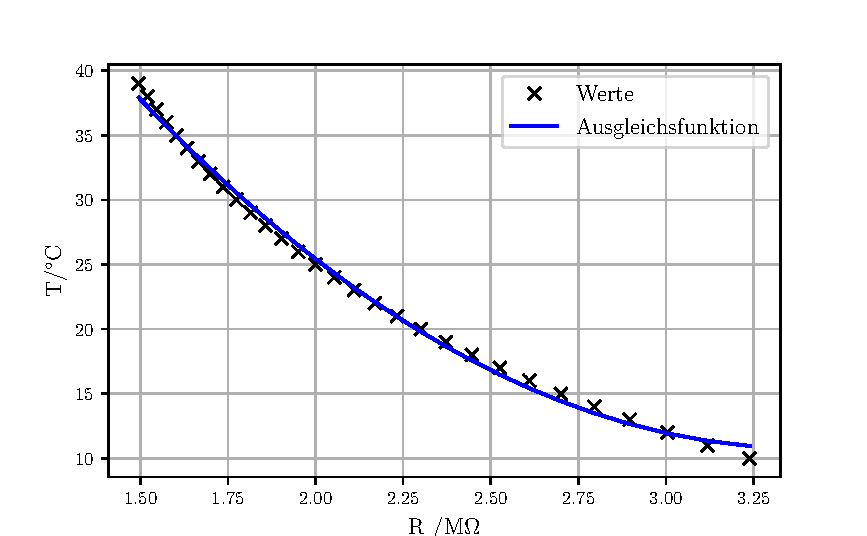
\includegraphics[width=0.8\textwidth]{build/plot1.pdf}
        \caption {Zusammenhang zwischen Widerstand und Temperatur.}
        \label{fig:plottemp}
\end{figure}

Nun kann aus \autoref{fig:Abb_2} die Viskosität der Luft für die Temperatur abgelesen werden.
Mithilfe des WebplotDigitizers \cite{Rohatgi2020} wird die Geradengleichung zu
\begin{align*}
       \eta = 0.0048 \cdot T + 1.7268 
\end{align*}
bestimmt.
Die berechneten Werte der Temperatur, Viskosität, sowie unkorrigierter Ladung und Radius der Öltröpfchen sind in \autoref{tab:unkorr} aufgelistet.

\begin{table}[H]
        \centering
        \caption{Berechnete Daten der Öltröpfchen (unkorrigiert).}
        \label{tab:unkorr}
        \sisetup{table-format=1.3}
        \begin{tabular}{SSSSS}
        \toprule
        {$R / \si{\mega\ohm}$}& {$T / \si{\celsius}$} &{$\eta_{Luft} / 10^{-5} \frac{\si{\newton\second}}{\si{\meter\squared}}$} & {r}& {q} \\
        \midrule
        1.992 & 25.60 & 1.8497 & & \\   
        1.990 & 25.64 & 1.8499 & & \\   
        1.986 & 25.73 & 1.8503 & & \\  
        1.980 & 25.85 & 1.8510 & & \\
        1.975 & 25.96 & 1.8514 & & \\ 
        1.970 & 26.07 & 1.8519 & & \\   
        1.967 & 26.13 & 1.8522 & & \\ 
        1.965 & 26.17 & 1.8524 & & \\ 
        1.958 & 26.32 & 1.8532 & & \\   
        1.951 & 26.48 & 1.8539 & & \\  
        1.950 & 26.50 & 1.8540 & & \\   
        1.948 & 26.54 & 1.8542 & & \\  
        1.947 & 26.56 & 1.8543 & & \\ 
        1.947 & 26.56 & 1.8543 & & \\
        1.939 & 26.74 & 1.8551 & & \\ 
        1.937 & 26.78 & 1.8553 & & \\ 
        1.934 & 26.85 & 1.8557 & & \\      
        1.930 & 26.93 & 1.8561 & & \\   
        1.930 & 26.93 & 1.8561 & & \\
        1.930 & 26.93 & 1.8561 & & \\ 
        \bottomrule
        \end{tabular}
\end{table}




1 2 13 15 22 weg 